\documentclass[11pt]{article}
% \pagestyle{empty}

\setlength{\oddsidemargin}{-0.25 in}
\setlength{\evensidemargin}{-0.25 in}
\setlength{\topmargin}{-0.9 in}
\setlength{\textwidth}{7.0 in}
\setlength{\textheight}{9.0 in}
\setlength{\headsep}{0.75 in}
\setlength{\parindent}{0.3 in}
\setlength{\parskip}{0.1 in}
\usepackage{epsf}
\usepackage{pseudocode}
\usepackage{amsmath}
\usepackage{amssymb}
\usepackage{mathtools}
\usepackage{listings}
\DeclarePairedDelimiter{\ceil}{\lceil}{\rceil}
\DeclarePairedDelimiter\floor{\lfloor}{\rfloor}
\usepackage{listings}
\usepackage{color}
 
\definecolor{codegreen}{rgb}{0,0.6,0}
\definecolor{codegray}{rgb}{0.5,0.5,0.5}
\definecolor{codepurple}{rgb}{0.58,0,0.82}
\definecolor{backcolour}{rgb}{0.95,0.95,0.92}
 
\lstdefinestyle{mystyle}{
  backgroundcolor=\color{backcolour},
  commentstyle=\color{codegreen},
  keywordstyle=\color{magenta},
  numberstyle=\tiny\color{codegray},
  stringstyle=\color{codepurple},
  basicstyle=\footnotesize,
  breakatwhitespace=false,
  breaklines=true,
  captionpos=b,
  keepspaces=true,
  numbers=left,
  numbersep=5pt,
  showspaces=false,
  showstringspaces=false,
  showtabs=false,
  tabsize=2
}
 
\lstset{style=mystyle}
% \usepackage{times}
% \usepackage{mathptm}

\def\O{\mathop{\smash{O}}\nolimits}
\def\o{\mathop{\smash{o}}\nolimits}
\newcommand{\e}{{\rm e}}
\newcommand{\R}{{\bf R}}
\newcommand{\Z}{{\bf Z}}
\DeclarePairedDelimiter\abs{\lvert}{\rvert}%
\DeclarePairedDelimiter\norm{\lVert}{\rVert}%

% Swap the definition of \abs* and \norm*, so that \abs
% and \norm resizes the size of the brackets, and the 
% starred version does not.
\makeatletter
\let\oldabs\abs
\def\abs{\@ifstar{\oldabs}{\oldabs*}}
%
\let\oldnorm\norm
\def\norm{\@ifstar{\oldnorm}{\oldnorm*}}
\makeatother
\title{CS 181: Practical 4}
\author{Helen Wu, James Kim, Spencer Kim}
\date{April 28, 2017}
\begin{document}
\maketitle

\section{Technical Approach}

Our objective in this practical was to have the machine learn how to play Swingy Monkey. We took several approaches to this, based around reinforcement learning. 

We needed to extract information out of the state dictionary to use as our representation of our current state for reinforcement learning. We chose to use the following information from the state dictionary: horizontal distance to the next tree, vertical distance from the top of the tree to the top of the monkey, and velocity. 

We also encountered the challenge of the large state space. As the practical specifications suggested, the state space was almost continuous, so we needed a way to decrease this. 

To deal with the large state space, we first attempted to use a neural network to model the Q function that maps state/actions to the Q table. However, to make the network easier to train, we designed the network so that the input was the flattened 7 feature state dictionary, and the output was a size 2 vector that held the Q values for the actions 0 and 1. The neural net was a 3 layered dense (70, 150, 80) feed-forward architecture. We also tried a much simpler model, with one layer of 150 neurons. It was trained using experience replay, which uses batches from previous data rather than the most recent one to train the neural network. This helps the neural net not fall into local minima. However, over enough iterations, the neural net will ultimately be trained over a majority of the experiences.

We also attempted to divide the possible values of each of these state values into discrete bins, so that a range of the values of each of the  One of our parameters that we chose to modify was the number of pixels in each of these bins (could also conceptualize this as modifying the number of bins). Two of the values that we tried were 20 pixels per bin and 50 pixels per bin. We predicted that using fewer pixels per bin would take longer to converge (because there are a lot more Q values to learn) but would yield a better result.

The first approach we tried was basic SARSA. We wanted to try on-policy learning because we reasoned that it allows for more exploration, which can lead to a more accurate convergence. This was a fair approach, which yielded results, but we wanted to find an algorithm that would lead to a better result.

The second approach we tried was basic Q-learning. Even though we had reasoning for using an on-policy, we considered that  in the case of this game, it may be a better approach to take the best action as we've currently predicted it (exploit) and not attempt to explore. This yielded much better results, especially when we adjusted our parameters.



\section{Data}
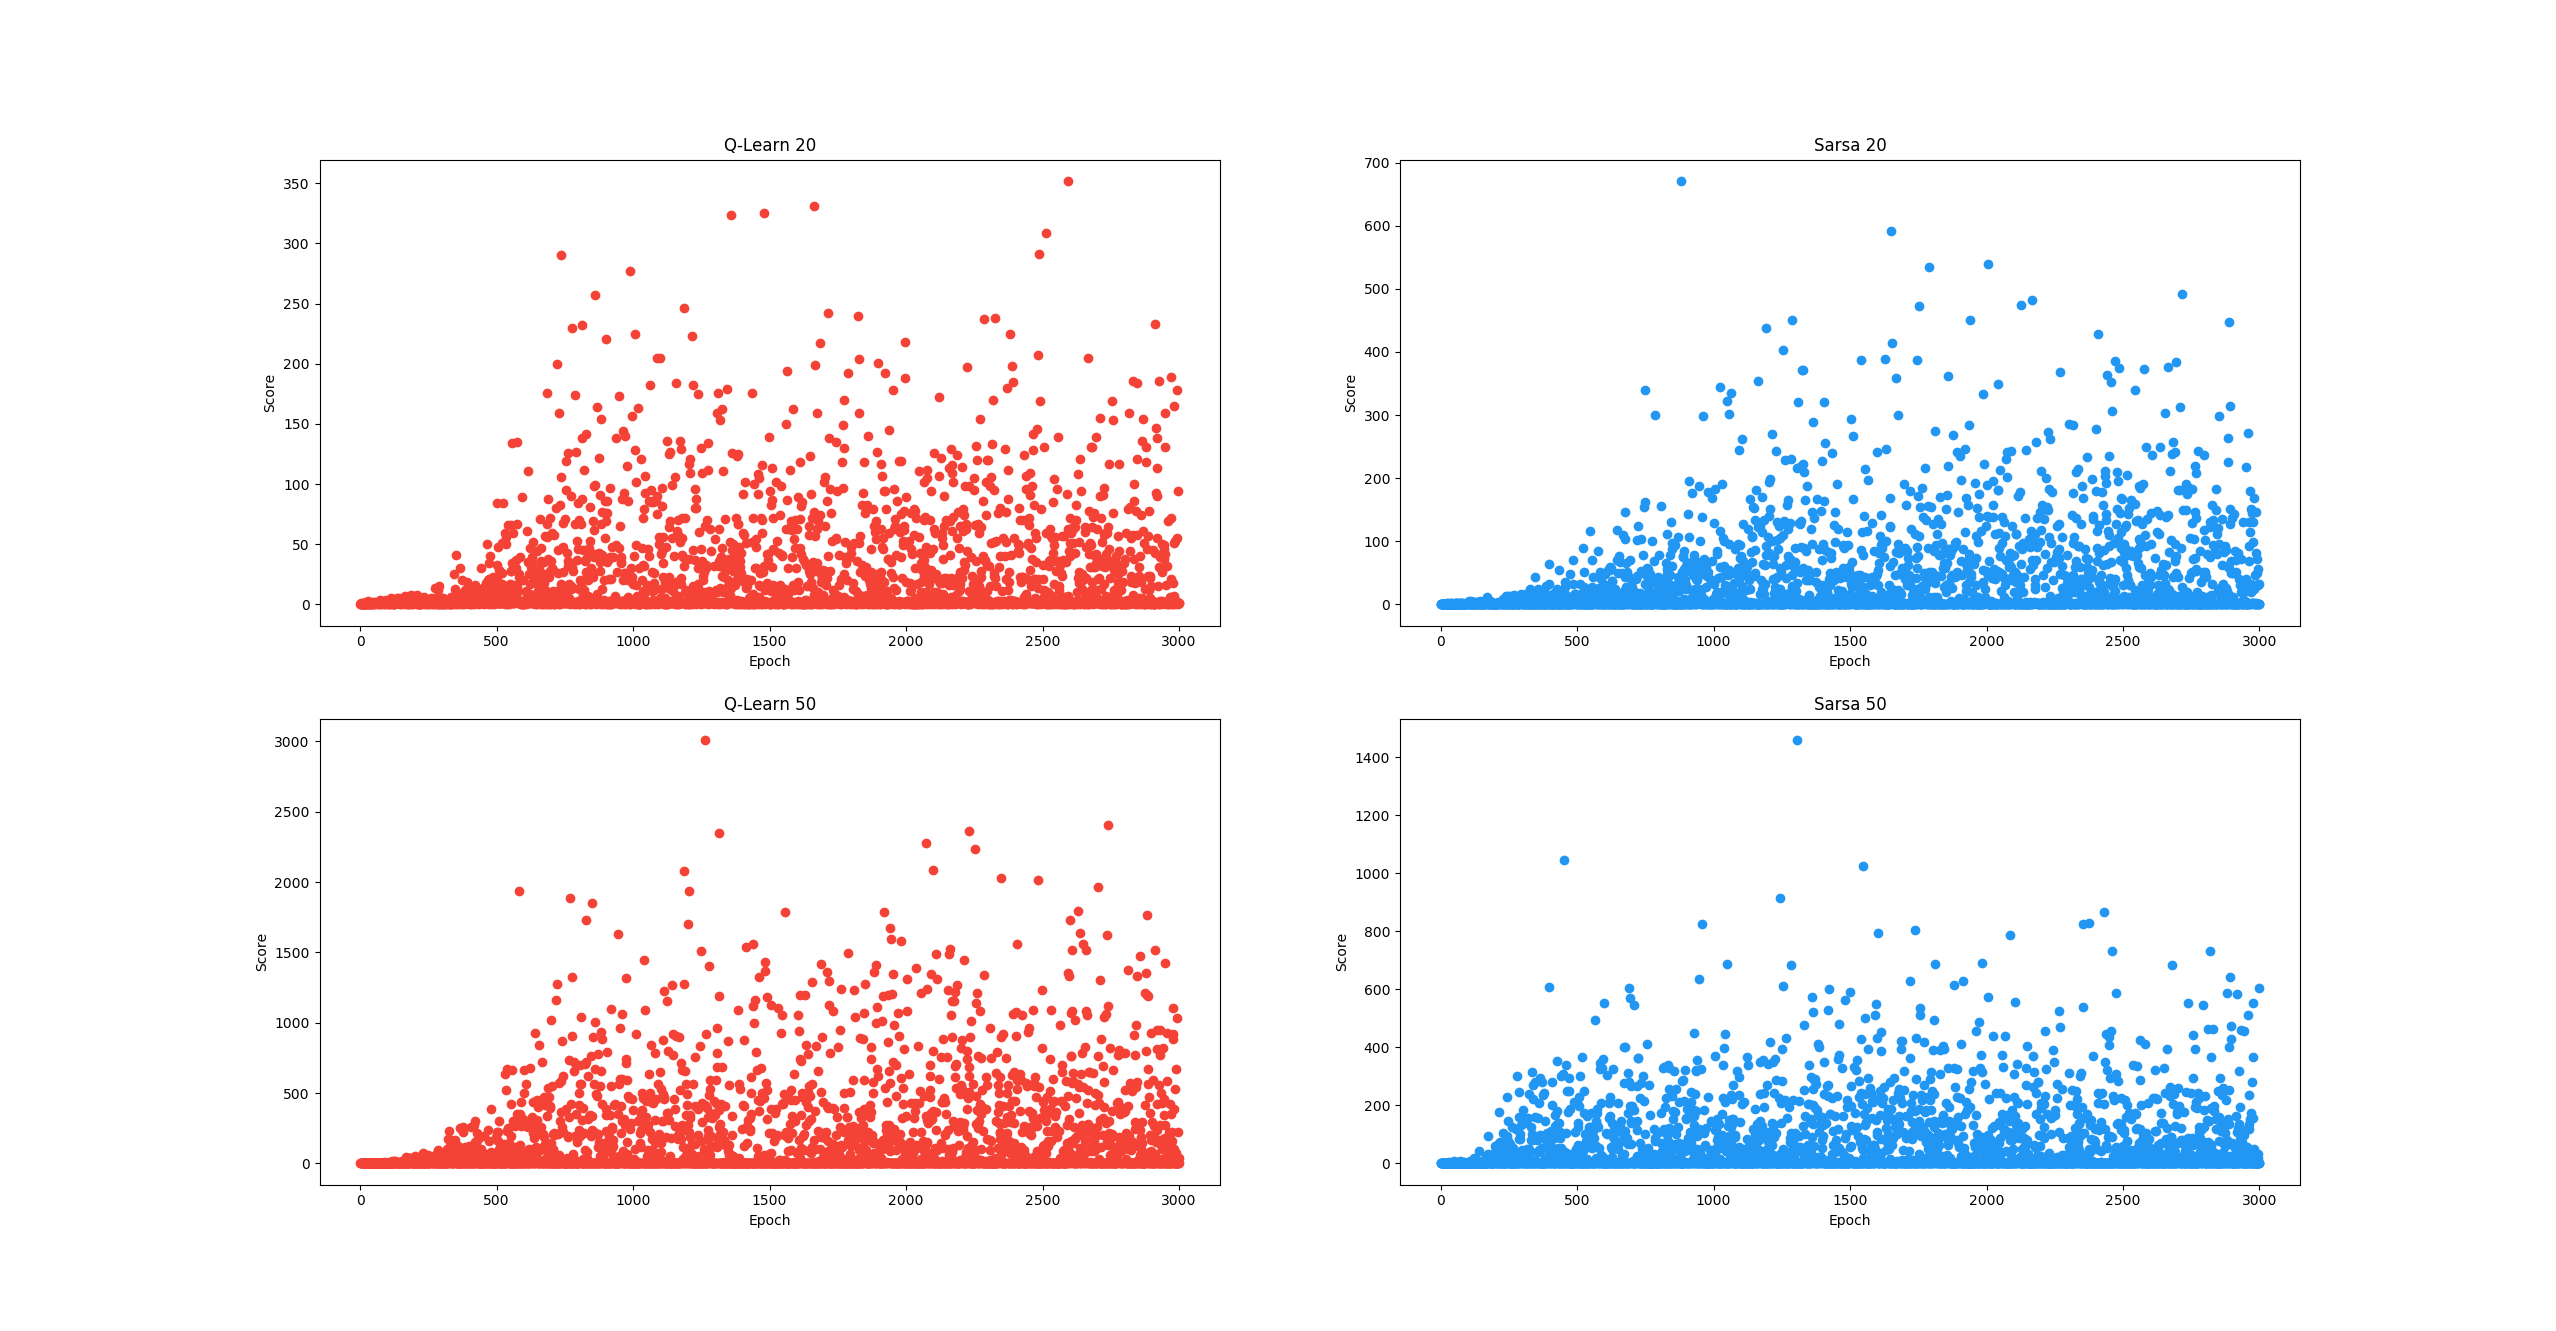
\includegraphics[width=20cm]{../figures/points.png}\\
Looking at the above data we notice that generally, for both Q-learning and SARSA, when using larger bins, and thus fewer states, we see faster convergence. This is likely due to the fact that when we have fewer states the need for exploration is diminished, and thus, the amount of exploration that is necessary in order to find a relatively effective state is decreased. We conjecture that both the Q-learning and SARSA algorithms had failed to reach a relatively optimal strategy after 3000 epochs, as we would expect that a relatively optimal strategy using more precise data would outpreform a relatively optimal strategy using less precise data. Thus, we would want to train the 20 pixels-per-bin algorithms for longer than the 50 pixels-per-bin. It is worth noting that despite the fact that all algorithms were given equivalent training epochs, the amount of time given to each algorhtm differed significantly. Using the Linux `time' method we recieved the following output:
\begin{lstlisting}
(cs181) $ time python std_runner.py qlearn 20
real  55m31.065s
user  65m52.556s
sys 14m29.203s

(cs181) $ time python std_runner.py sarsa 20
real  71m8.945s
user  87m18.156s
sys 18m25.350s

(cs181) $ time python std_runner.py sarsa 50
real  109m42.988s
user  151m46.082s
sys 28m8.916s

(cs181) $ time python std_runner.py qlearn 50
real  244m46.278s
user  356m23.755s
sys 63m56.786s
\end{lstlisting}
This is because high-scoring runs take longer than low-scoring runs, thus it is more reasonable that it might initially appear to give the 20 pixel-per-bin algorithms additional training epochs.

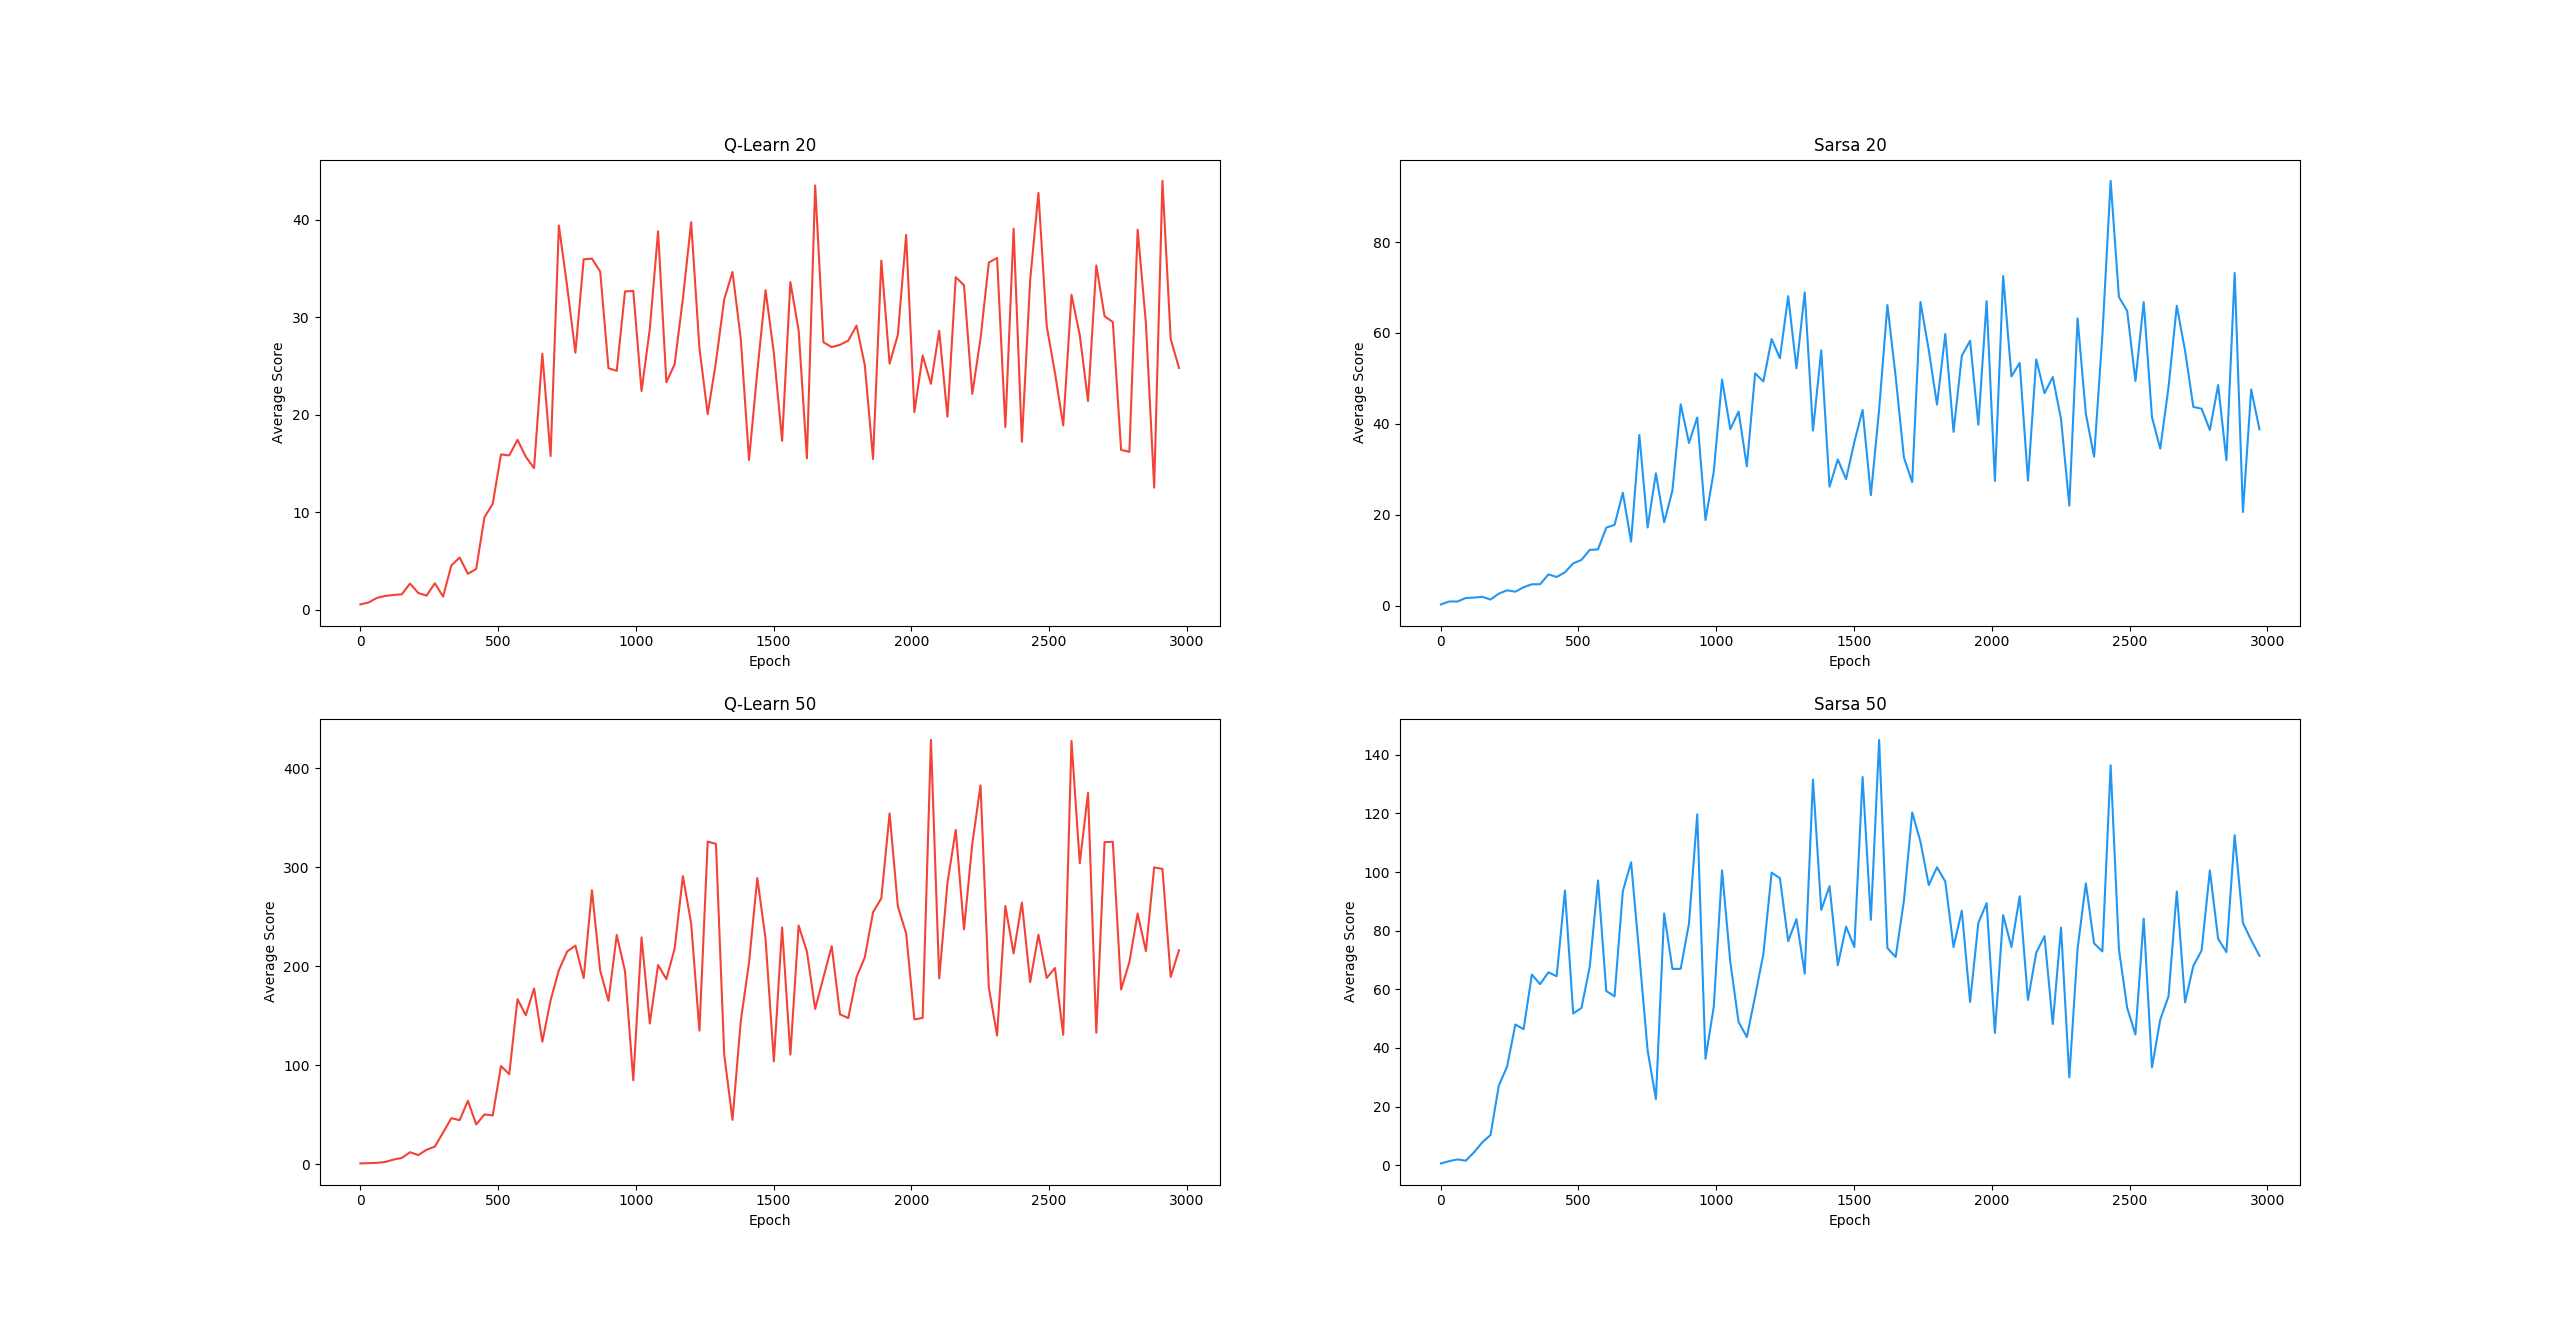
\includegraphics[width=20cm]{../figures/avg.png}\\
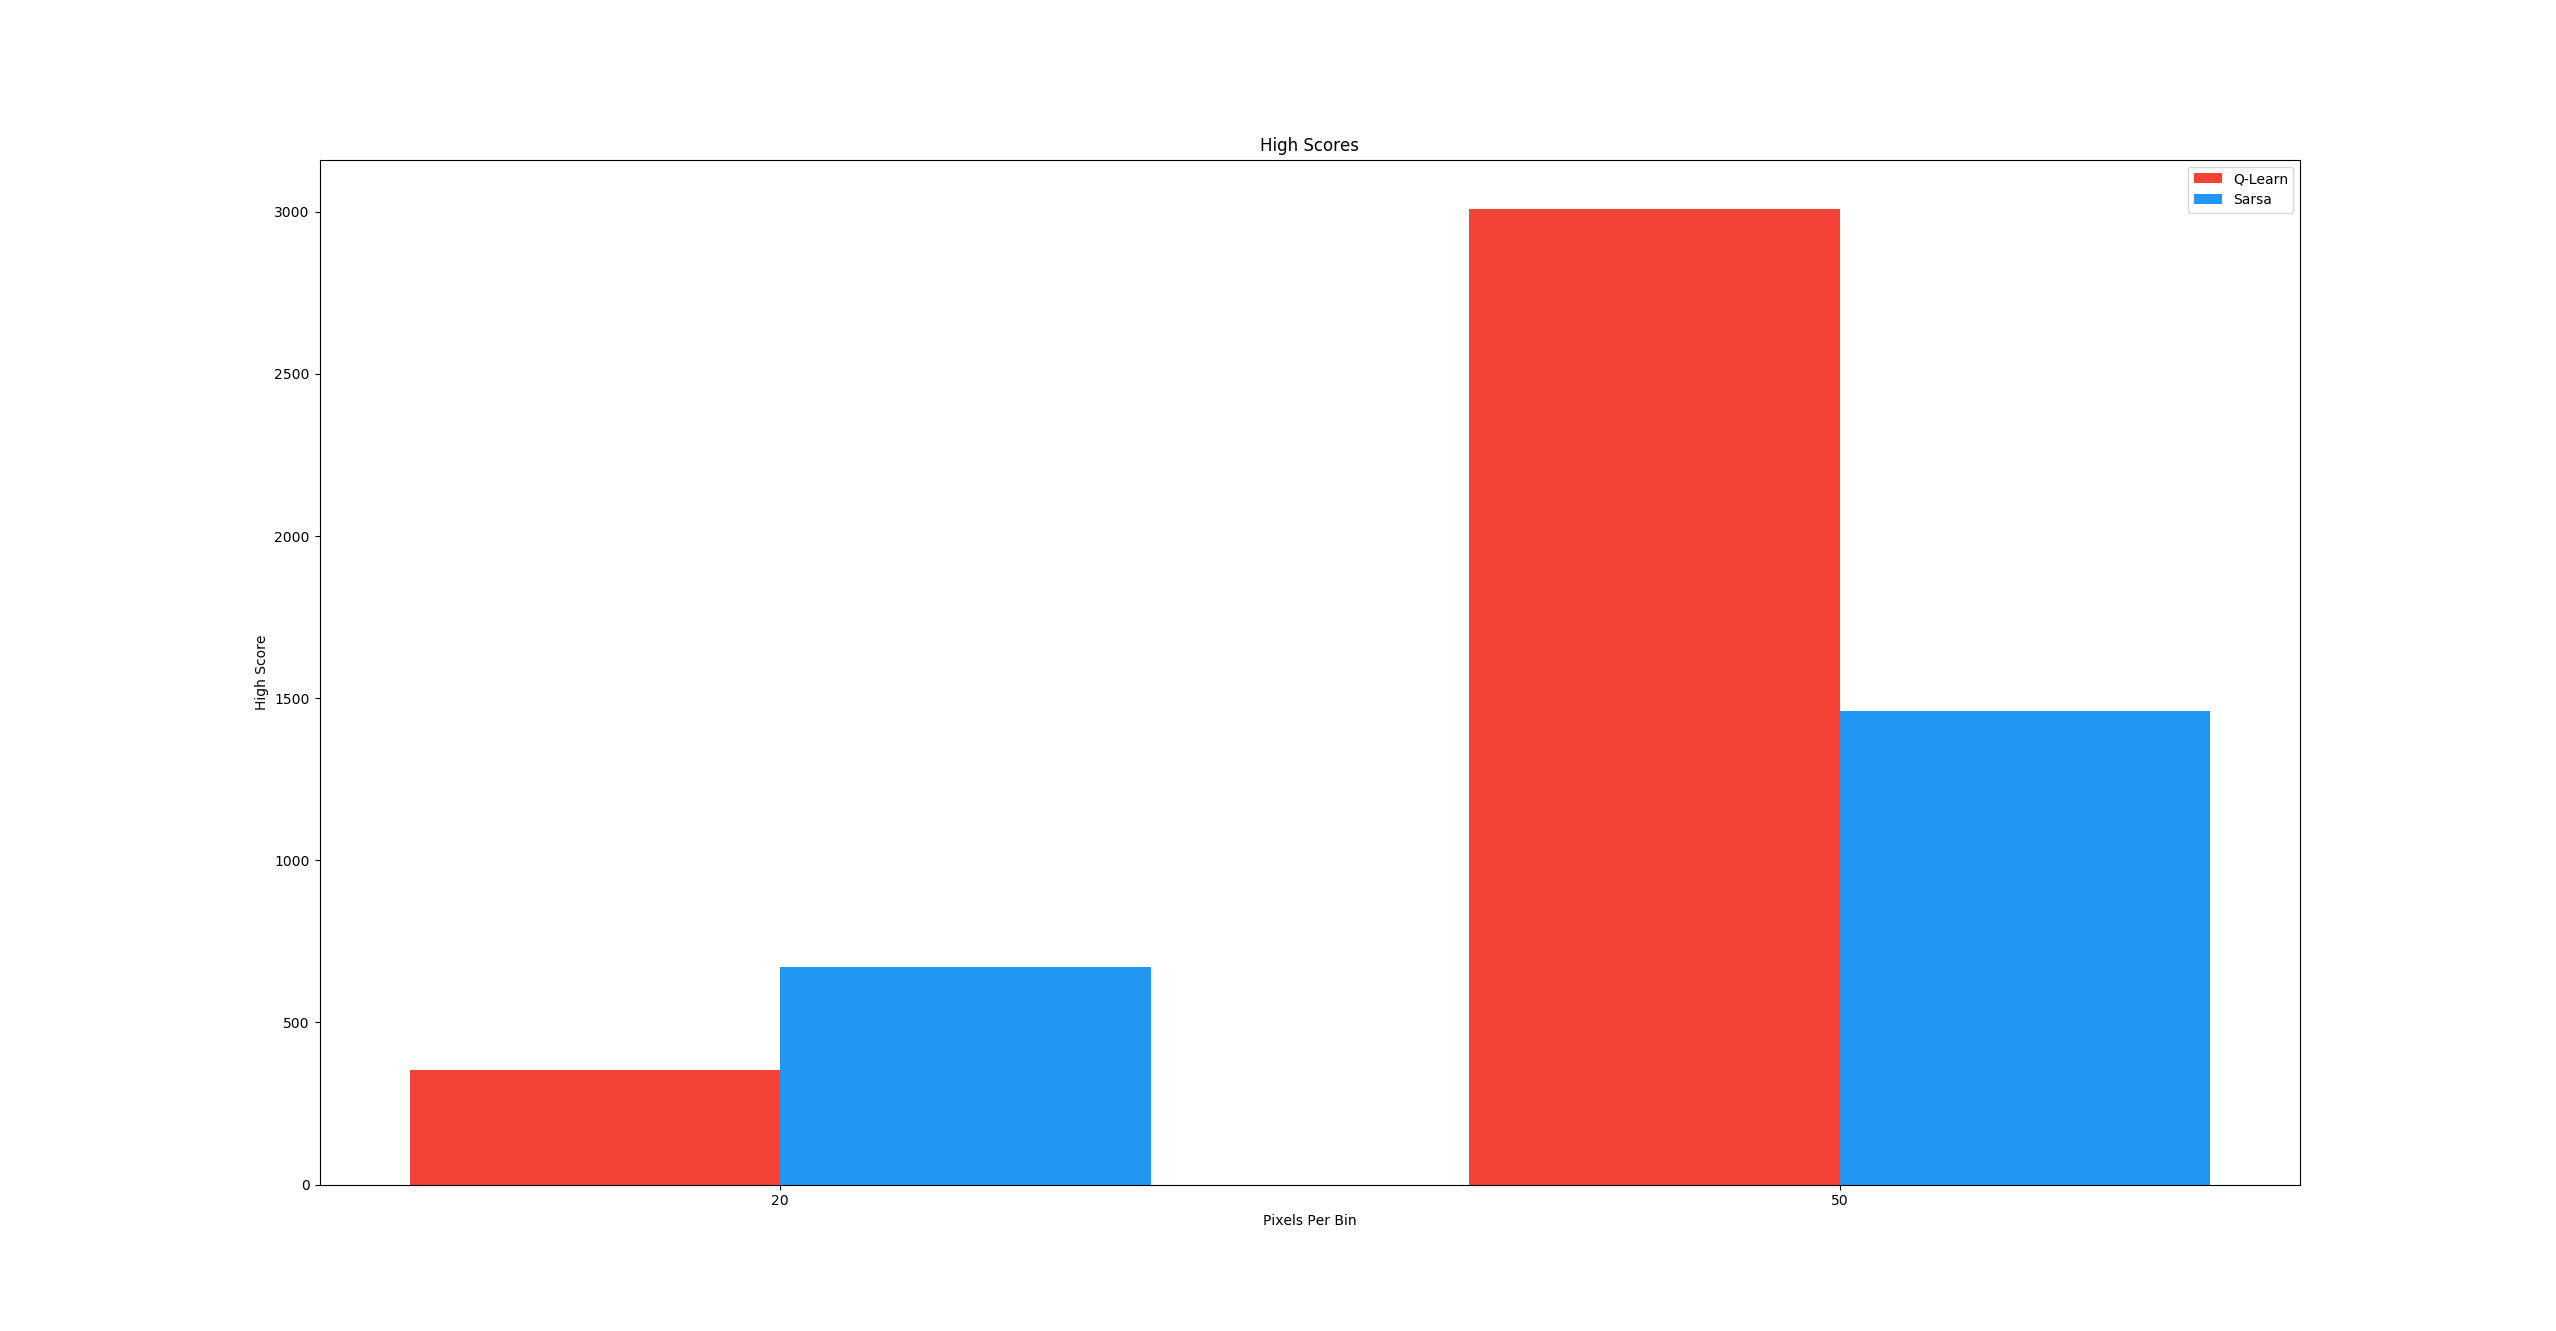
\includegraphics[width=20cm]{../figures/hiscores.png}\\

\section{Discussion}

The neural net was not particularly effective in representing the Q function. It seemed to learn quite quickly for perhaps the first 100 epochs, but then would begin to overfit, cause the monkey to immediately crash into the ceiling. We tried various configurations of the neural network, and the batch size in the experience replay, but ultimately we were only able to improve the scores to a maximum of 20 and mean of 1.52 after 1000 epochs. We believe that the problem was due to the neural network being too complex and ultimately overfitting. Therefore, we tried a much simpler model with a single layer of 150 neurons. It performed better by yielding a maximum of 52 and mean of 3.21 after 1000 epochs. However, we also think that neural nets are slow to converge, and much more prone to overfitting, and therefore we should try using some other form of state representation.

When analyzing the performance of these algorithms we noticed a large amount of variance, which is understandable due to the imprecise nature of our model as well as the shifting nature of the game (its `gravity' value is non-constant). However, even so we saw distinct trends. In the 20 pixel-per-bin algorithms we saw that SARSA outperformed Q-learning significantly, whereas in the 50 pixel-per-bin algorithms we saw the reverse. We think this was caused by the fact that since SARSA converges more quickly to an optimum, when training on a larger state space with a small amount of training data it is able to outperform Q-learning (a trend that we observed in both bin sizes), however when the algorithm is given enough time to converge to an optimum, Q-learning will outperform, as it is an off-policy model and thuw will better converge to an optimal policy.


\end{document}

